\documentclass{beamer}

\usepackage[orientation=landscape,size=a0,scale=1.4,debug]{beamerposter}
\mode<presentation>{\usetheme{mlr}}

\usepackage[utf8]{inputenc} % UTF-8
\usepackage[english]{babel} % Language
\usepackage{hyperref} % Hyperlinks
\usepackage{ragged2e} % Text position
\usepackage[export]{adjustbox} % Image position
\usepackage[most]{tcolorbox}
\usepackage{listings} % for R code
\lstset{language=R,
    basicstyle=\small\ttfamily,
    stringstyle=\color{DarkGreen},
    otherkeywords={0,1,2,3,4,5,6,7,8,9},
    morekeywords={TRUE,FALSE},
    deletekeywords={data,frame,length,as,character},
    keywordstyle=\color{blue},
    commentstyle=\color{DarkGreen},
}

\title{mlr3 :\,: CHEAT SHEET} % Package title in header, \, adds thin space between ::
\newcommand{\packagedescription}{ % Package description in header
	The \textbf{mlr3} package provides a framework for classification, regression and other machine learning tasks.
}

\newlength{\columnheight} % Adjust depending on header height
\setlength{\columnheight}{84cm} 

\newtcolorbox{codebox}{%
	sharp corners,
	leftrule=0pt,
	rightrule=0pt,
	toprule=0pt,
	bottomrule=0pt,
	hbox}

\newtcolorbox{codeboxmultiline}[1][]{%
	sharp corners,
	leftrule=0pt,
	rightrule=0pt,
	toprule=0pt,
	bottomrule=0pt,
	#1}

\begin{document}
\begin{frame}[fragile]{}
\begin{columns}
	\begin{column}{.245\textwidth}
		\begin{beamercolorbox}[center]{postercolumn}
			\begin{minipage}{.98\textwidth}
				\parbox[t][\columnheight]{\textwidth}{
					\begin{myblock}{Resources}
						\begin{itemize}
							\item \href{https://mlr3book.mlr-org.com/index.html}{mlr3book}
							\item \href{https://github.com/mlr-org}{mlr-org on GitHub} 
						\end{itemize}
					\end{myblock}
						\begin{myblock}{Packages}
										\vfill
						\begin{itemize}
							\item \href{https://github.com/mlr-org/mlr3pipelines}{mlr3pipelines} - Dataflow Programming
							\item \href{https://github.com/mlr-org/mlr3tuning}{mlr3tuning} - Tuning Methods
							\item \href{https://github.com/mlr-org/mlr3filters}{mlr3filters} - Feature Selection Filters
							\item \href{https://github.com/mlr-org/mlr3survival}{mlr3survival} - Survival analysis
							\item \href{https://github.com/mlr-org/mlr3fswrap}{mlr3fswrap} - Wrapper feature selection
							\item \href{https://github.com/mlr-org/mlr3learners}{mlr3learners} - Recommended learners
							\item \href{https://github.com/mlr-org/mlr3viz}{mlr3viz} - Visualizations
							\item \href{https://github.com/mlr-org/mlr3ordinal}{mlr3ordinal} - Ordinal Regression
						\end{itemize}
					\end{myblock}

					\begin{myblock}{Intro \& Workflow}
					The mlr3 package provides R6 classes for the essential building
					blocks of this machine learning workflow:
					
          1. A \textbf{task} encapsulates the data along with additional information, such as 
          what the prediction target is.
          
          2. A \textbf{learner} encapsulates one of R's many machine learning algorithms and allows 
          to train models and make predictions.
          Most learners have hyperparameters.
          
          3. A \textbf{measure} computes a numeric score based on predicted and ground-truth values 
          and their difference.
          
          4. A \textbf{resampling} specifies a series of train and test sets.
          \end{myblock}
    
				  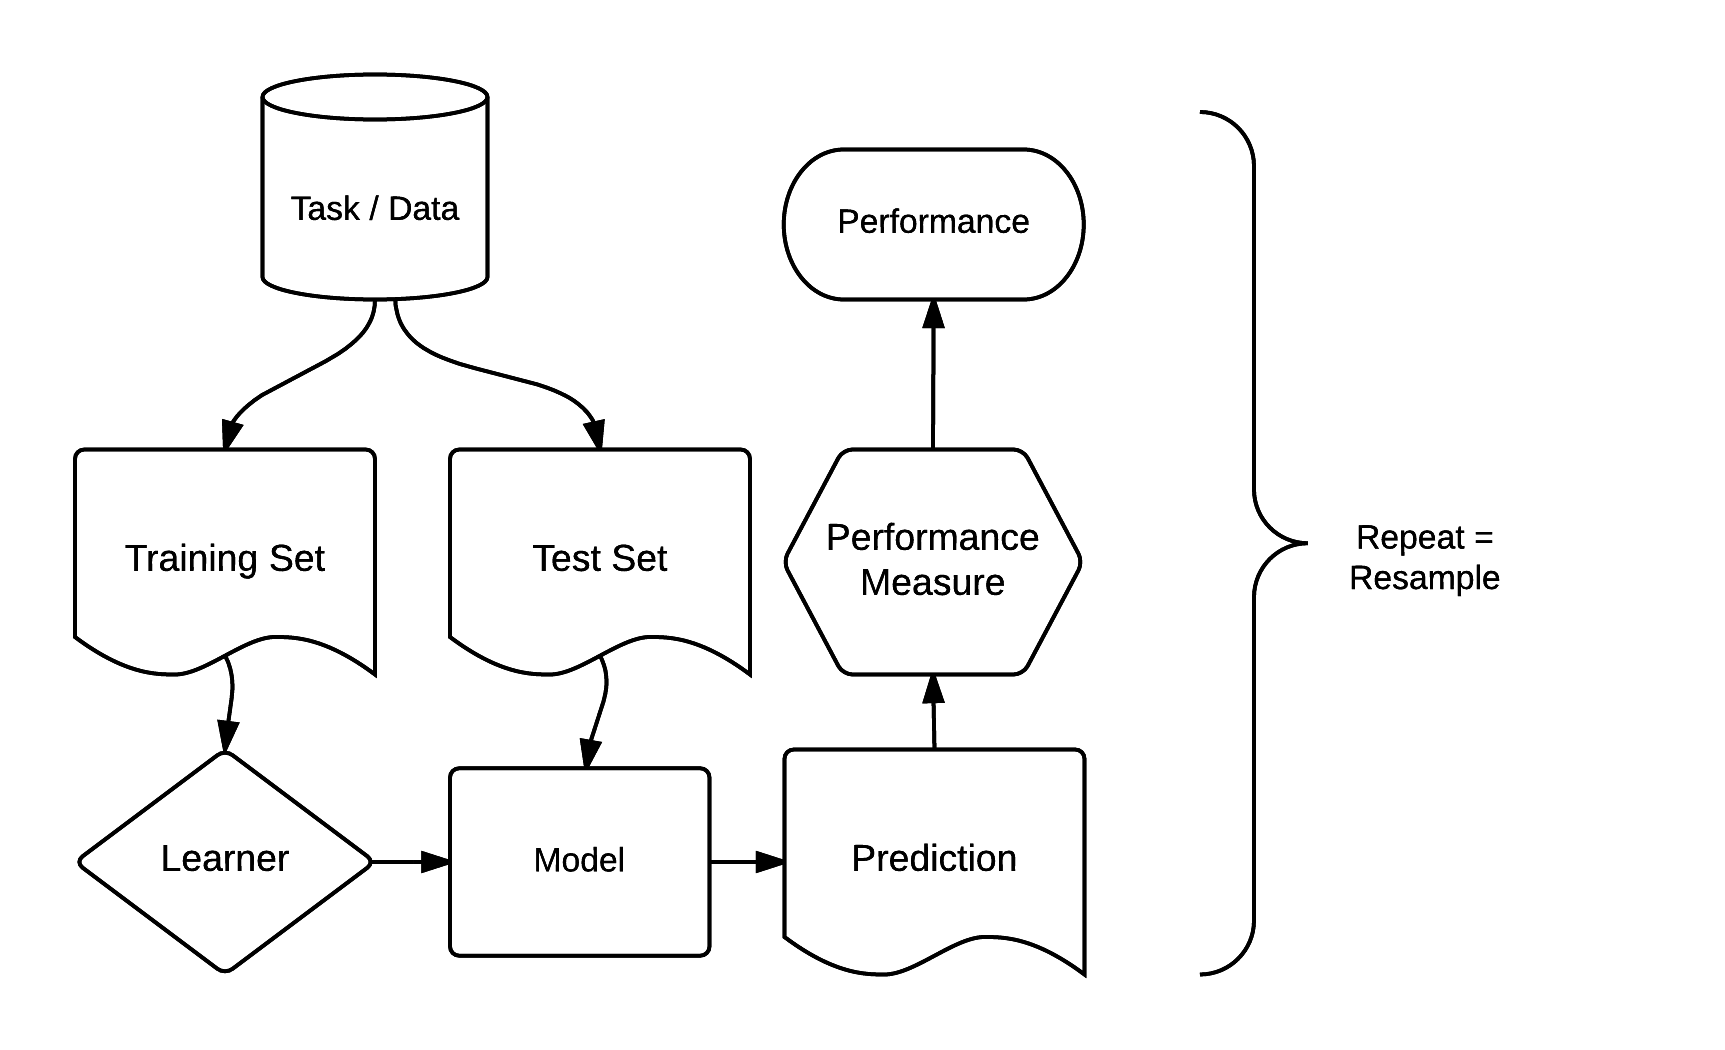
\includegraphics[width=\textwidth]{img/ml_abstraction.png}
				}
			\end{minipage}
		\end{beamercolorbox}
	\end{column}
	\begin{column}{.245\textwidth}
		\begin{beamercolorbox}[center]{postercolumn}
			\begin{minipage}{.98\textwidth}
				\parbox[t][\columnheight]{\textwidth}{
									\begin{myblock}{Task}
						Tasks objects store data (\textit{backend}) and additional meta-data for machine learning problems. A \textit{backend} allows fine-grained control over how data is accessed. If you simply provide the dataset, it is automatically converted to a \textit{DataBackendDataTable}.
						\\
						\begin{codebox}
							task = \textbf{TaskClassif}\$new(backend, target)
						\end{codebox}
						\hspace*{1ex}The \textit{target} is handed over as character value. For classification, the name of the target column is a label with only few distinct values.
						\\
						\begin{codebox}
							task = \textbf{TaskRegr}\$newt(backend, target)
						\end{codebox}
						\hspace*{1ex}The \textit{target} is a numeric quantity.
						\\
						\begin{codebox}
							task = \textbf{mlr\_tasks}\$\textbf{get}(key)
						\end{codebox}
						\hspace*{1ex}Get predefined task by \textit{key} from mlr\_task dictionary. The key (character value) identifies these tasks. 
						\\
						\begin{codebox}
							task\$\textbf{data}()
						\end{codebox}
						\hspace*{1ex}Retrieves stored data.
						\\
						\begin{codebox}
							task\$\textbf{set\_col\_role}(cols, new\_roles)
						\end{codebox}
						\begin{codebox}
							task\$\textbf{set\_row\_role}(rows, new\_roles)
						\end{codebox}
						\hspace*{1ex} Assign role (\textit{new\_roles}) to \textit{cols} / \textit{rows}. These task methods change the view on the data and can be used to subset the task.
						\\
						\begin{codebox}
							task\$\textbf{select}(cols)
						\end{codebox}
						\hspace*{1ex}Subsets the task based on feature names (\textit{cols}).
						\\
						\begin{codebox}
							task\$\textbf{filter}(rows)
						\end{codebox}
						\hspace*{1ex}Subsets the task based on row ids (\textit{rows}).
					\end{myblock}
					\vfill
				}
			\end{minipage}
		\end{beamercolorbox}
	\end{column}
	\begin{column}{.245\textwidth}
		\begin{beamercolorbox}[center]{postercolumn}
			\begin{minipage}{.98\textwidth}
				\parbox[t][\columnheight]{\textwidth}{
					\begin{myblock}{Learner}
						Learner objects provide a unified interface to machine learning algorithms.
						\\
						\begin{codebox}
							learner = \textbf{mlr\_learners}\$\textbf{get}(key)
						\end{codebox}
						\hspace*{1ex}Get learner by \textit{key} from mlr\_learner dictionary.
						\\
						\begin{codebox}
							learner\$\textbf{param\_set}
						\end{codebox}
						\hspace*{1ex}Returns a description of hyperparameter settings.
					\end{myblock}
				\begin{myblock}{Train \& Predict}
						Training fits a model to a given task. 
						\\
						\begin{codebox}
							train\_set = \textbf{sample}(task\$nrow, 0.8 * task\$nrow)
						\end{codebox}
						\hspace*{1ex}Get train set.
						\\
						\begin{codebox}
							test\_set = \textbf{setdiff}(seq\_len(task\$nrow), train\_set)
						\end{codebox}
						\hspace*{1ex}Get test set.
						\\
						\begin{codebox}
							learner\$\textbf{train}(task, row\_ids = train\_set)
						\end{codebox}
						\hspace*{1ex}Train model with the \textit{train\_set}.
						\\
						\begin{codebox}
							prediction = learner\$\textbf{predict}(task, row\_ids = test\_set)
						\end{codebox}
						\hspace*{1ex}Predict \textit{test\_set} with model.
						\\
						\begin{codebox}
							measure = \textbf{mlr\_measures}\$\textbf{get}(key)
						\end{codebox}
						\hspace*{1ex}Get measure by \textit{key} from mlr\_measure dictionary.
						\\
						\begin{codebox}
							prediction\$\textbf{score}(measure)
						\end{codebox}
						\hspace*{1ex}Access performance with \textit{measure}.
					\end{myblock}
										}
			\end{minipage}
		\end{beamercolorbox}
	\end{column}
		\begin{column}{.245\textwidth}
		\begin{beamercolorbox}[center]{postercolumn}
			\begin{minipage}{.98\textwidth}
				\parbox[t][\columnheight]{\textwidth}{
					\begin{myblock}{Resampling}
						Resampling is used to assess the performance of a learning algorithm.
						\\[\baselineskip]
						\begin{minipage}{\textwidth}
							\begin{columns}[T]
								\begin{column}{0.2\textwidth}
									
\includegraphics[width=\textwidth]{img/cross_validation.png}
								\end{column}
								\begin{column}{0.8\textwidth}
										\begin{codebox}
										resampling = \textbf{mlr\_resamplings}\$\textbf{get}(key)
										\end{codebox}
										\hspace*{1ex}Get resampling strategy by \textit{key} from mlr\_resamplings \hspace*{1ex}dictionary.
								\end{column}
							\end{columns}
						\end{minipage}
						\\[\baselineskip]
						\begin{codebox}
							resampling\$\textbf{instantiate}(task)
						\end{codebox}
						\hspace*{1ex}Apply splitting on \textit{task}.
						\\
						\begin{codebox}
							rr = \textbf{resample}(task, learner, resampling)
						\end{codebox}
						\hspace*{1ex}Executes resampling.
						\\
						\begin{codebox}
							rr\$\textbf{performance}(measure)
						\end{codebox}
						\hspace*{1ex}Extract performance of individual resampling iterations with \textit{measure}.
					\end{myblock}
				\begin{myblock}{Benchmarking}
						Benchmarking is used to compare the performance of different learners on multiple task and/or different resampling schemes.
						\\
						\begin{codeboxmultiline}[width=21.95cm]
							design = \textbf{expand\_grid}(\\
							\hspace*{1ex}tasks = mlr\_tasks\$mget(key),\\
							\hspace*{1ex}learners = mlr\_learners\$mget(key),\\
							\hspace*{1ex}resamplings = mlr\_resamplings\$mget(key))
						\end{codeboxmultiline}
						\hspace*{1ex}Create benchmark design.
						\\
						\begin{codebox}
							bmr = \textbf{benchmark}(design)
						\end{codebox}
						\hspace*{1ex}Execute benchmark with \textit{design}.
						\\
						\begin{codebox}
							bmr\$\textbf{aggregate}(measure)
						\end{codebox}
						\hspace*{1ex}Calculate and aggregate performance.
					\end{myblock}\vfill
				}
			\end{minipage}
		\end{beamercolorbox}
	\end{column}
\end{columns}
\end{frame}
\end{document}
